% Условная компиляция для самостоятельной работы
\ifdefined\mainfile
    % Если это часть основного файла, не добавляем начало и конец документа
\else
    \documentclass[12pt, a4paper]{report}
    \usepackage{/Users/vladbelousov/Desktop/Semestr_4-FP-NSU/Настройка/library}
    \usepackage[utf8]{inputenc} % Подключение поддержки UTF-8
    \begin{document}
\fi

%%-------------------------------%%



\section{Дифракция плоской монохроматической волны на длинной щели}

Интеграл Кирхгофа для разложения по цилиндрическим волнам:

\[ E_p = \sqrt{\frac{k}{2 \pi i } } \int_{-\infty}^{\infty}   E(x' ) \frac{e^{i k R } }{\sqrt{R}} d x ' \cos \theta  \] 
\[ R = \sqrt{(x -x ' ) ^2 + z ^2 } = \sqrt{x ^2 + z ^2 - 2 x x' + (x' ) ^2 } \approx R_p -\frac{x}{R_p }x '      + \cancel{ o\left( \frac{(x') ^2 }{R_p}  \right)} \] 
, где \( x ^2+ z ^2 = R_p ^2  \) ,а \( o\left( \displaystyle \frac{(x') ^2 }{R_p}  \right) \) - в приближении Фраугофера равно нулю \( \left( \displaystyle  \frac{d ^2 }{\lambda R_p } \ll 1  \right) \).

\[ E_p = \sqrt{\frac{k}{ i R_p} } e^{ i k R_p } \underbrace{\left( \frac{1}{\sqrt{2 \pi } } \int_{-\infty}^{\infty}  E(x' ) e^{ - i k_x x ' } dx '    \right)}_{= \hat{E } (k_x)} \cos  \theta = \sqrt{\frac{k}{i R_p } } \hat{E } (k_x )\cos \theta  \] 
, где \( \displaystyle  k_x = k \frac{x}{R_p}  \) 

\begin{center}
    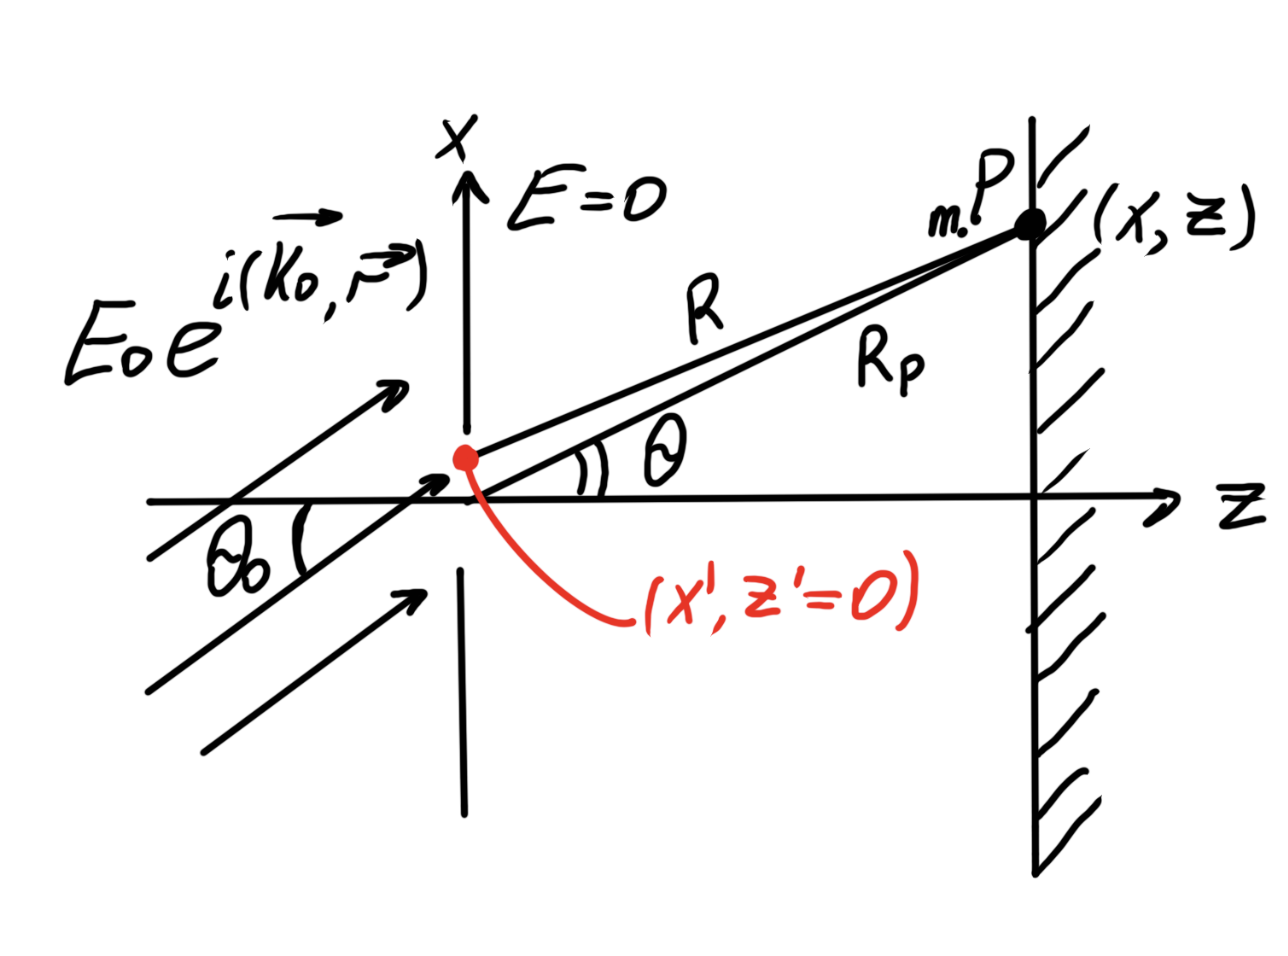
\includegraphics[width=0.5\textwidth]{/Users/vladbelousov/Desktop/Semestr_4-FP-NSU/ЭиО/Лекции_по_дням/image/135.png}
\end{center}
Падающая волна  под углом \( \theta_0 \)  имеет: \( \vec{k }_0  = (k_{0x } , 0 , k_{0z} ) , \text{ }  |\vec{k } _0   | = |\vec{k } | \) 
\[ E_0 e^{ ik_{0x }x'  + i k_{0z } z'  }  \Leftarrow E_0 e^{i (\vec{k } _0 , \vec{r} )} \] 
, где \( z ' = 0 \), а \( k_{0x} = k \sin \theta_0  \) 

\[ \hat{E } (k_x ) = \frac{1}{\sqrt{2 \pi}} \int_{- \frac{d}{2 } }^{\frac{d}{2 }  } E_0 e^{ i k \sin \theta_0 x' } e^{ - ik \sin \theta x } d x' = \frac{1}{\sqrt{2 \pi}}    E_0 \int_{- \frac{d}{2 } }^{\frac{d}{2 }  } e^{ i \Delta k_x x' }dx ' = \frac{ E_0}{\sqrt{ 2 \pi } } \frac{d e^{ i \Delta k_x \frac{d}{2 } }- e^{ - i \Delta k_x \frac{d}{2 } }  }{2 i \Delta k_x \frac{d}{2} }   \] 
\[=\frac{E_0 d }{\sqrt{2 \pi }}  \mathrm{sinc } \left( \Delta k_x \frac{d}{2 }  \right)  \] 

\[ I = \frac{\left\lvert  E_p    \right\rvert ^2 }{2 } = \frac{k }{R_p } \frac{ d ^2 }{2 \pi } \frac{\left\lvert E_0  \right\rvert ^2}{2 } \mathrm{sinc } ^2 \left( \Delta k_x \frac{d}{2 }  \right) \cos ^2 \theta =      \frac{ d ^2 }{\lambda R_p } I_0 \mathrm{sinc } ^2 \left(  \frac{kd }{2 }  (\sin \theta_0 - \sin \theta) \right)  \cos  ^2 \theta \] 
, где \( \displaystyle  I_0 = \frac{\left\lvert E_0  \right\rvert ^2}{2}  \), а \(\displaystyle  P_{\text{Ф} } = \frac{d ^2 }{ \lambda R_p}   \) 

\begin{center}
    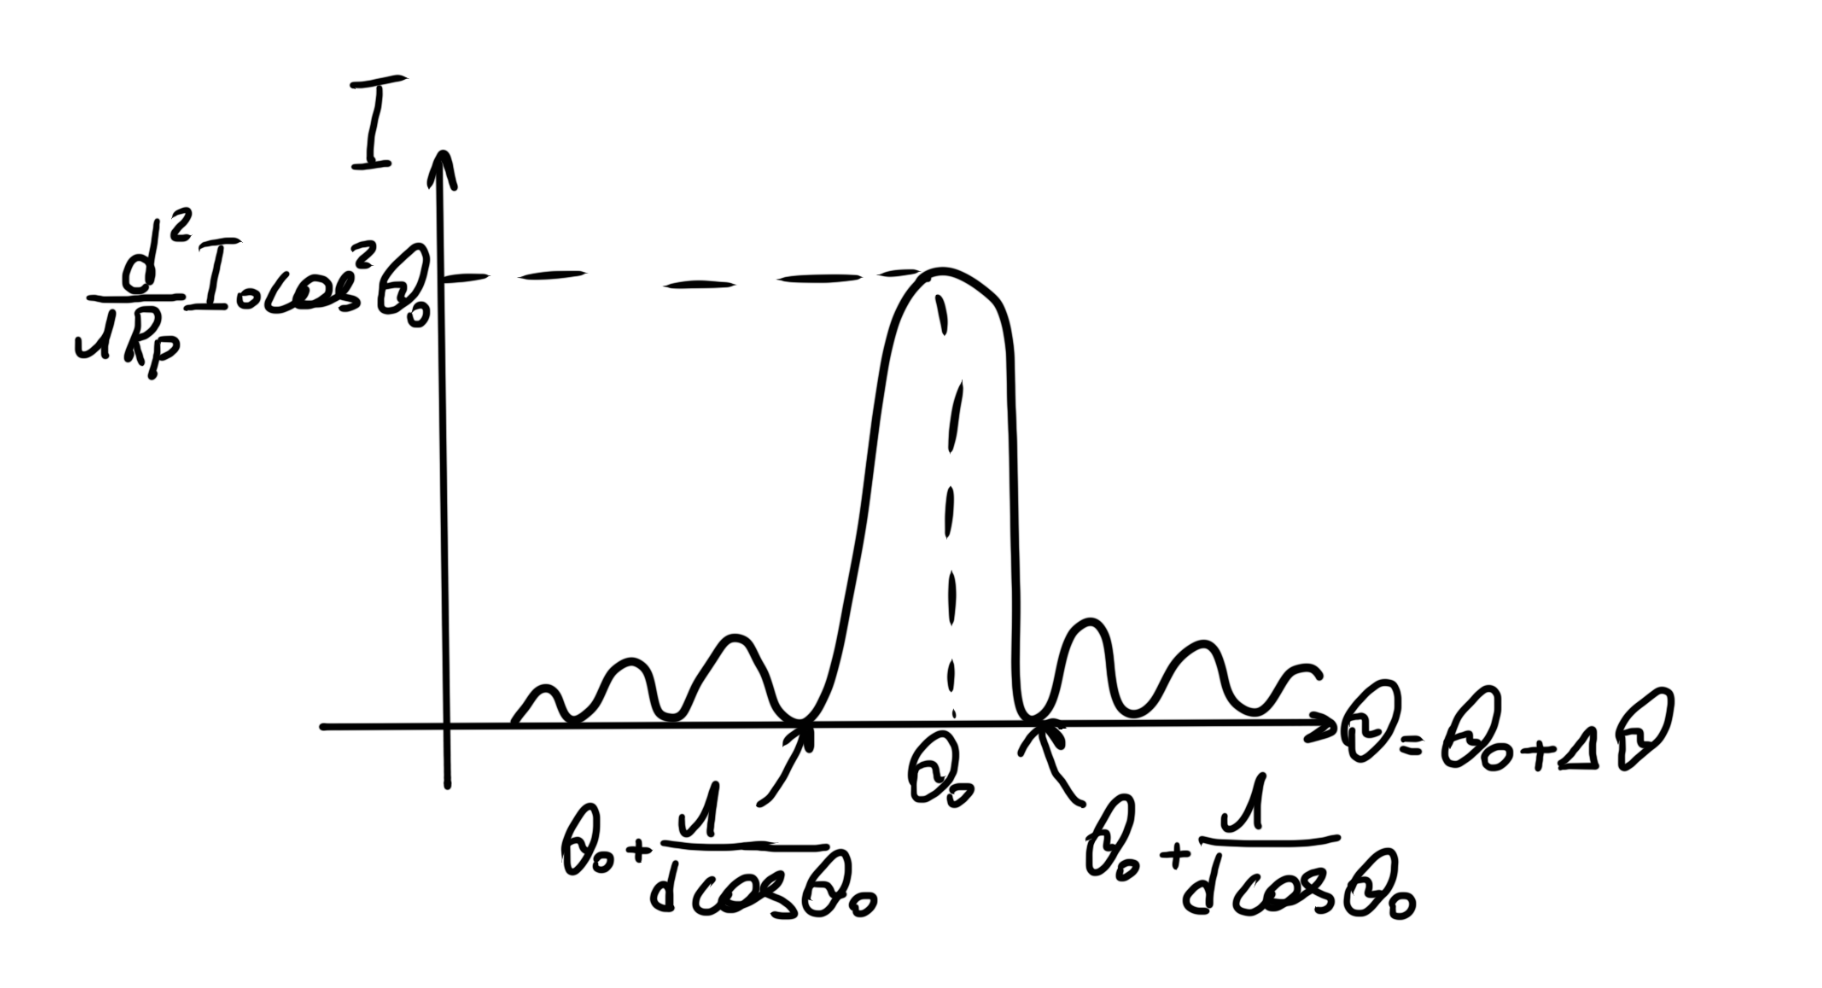
\includegraphics[width=0.7\textwidth]{/Users/vladbelousov/Desktop/Semestr_4-FP-NSU/ЭиО/Лекции_по_дням/image/136.png}
\end{center}

Первое обращение в "0" вблизи максимума  \( I(\theta) \). 

\[ \frac{kd }{2 } (\sin \theta_0 - \sin (\theta_0 + \Delta \theta)) = \pm  \pi  \] 
\[ \sin \theta_0 - \sin \theta_0 \underbrace{\cos \Delta \theta}_{\approx 1} - \cos  \theta_0 \underbrace{\sin  \Delta \theta}_{ \approx \Delta \theta} = \pm  \frac{\lambda}{d} \Rightarrow \Delta \theta = \frac{\lambda}{ d \cos \theta_0}   \] 

Дифракционная картина в фокальной плоскости линзы: 

\begin{center}
    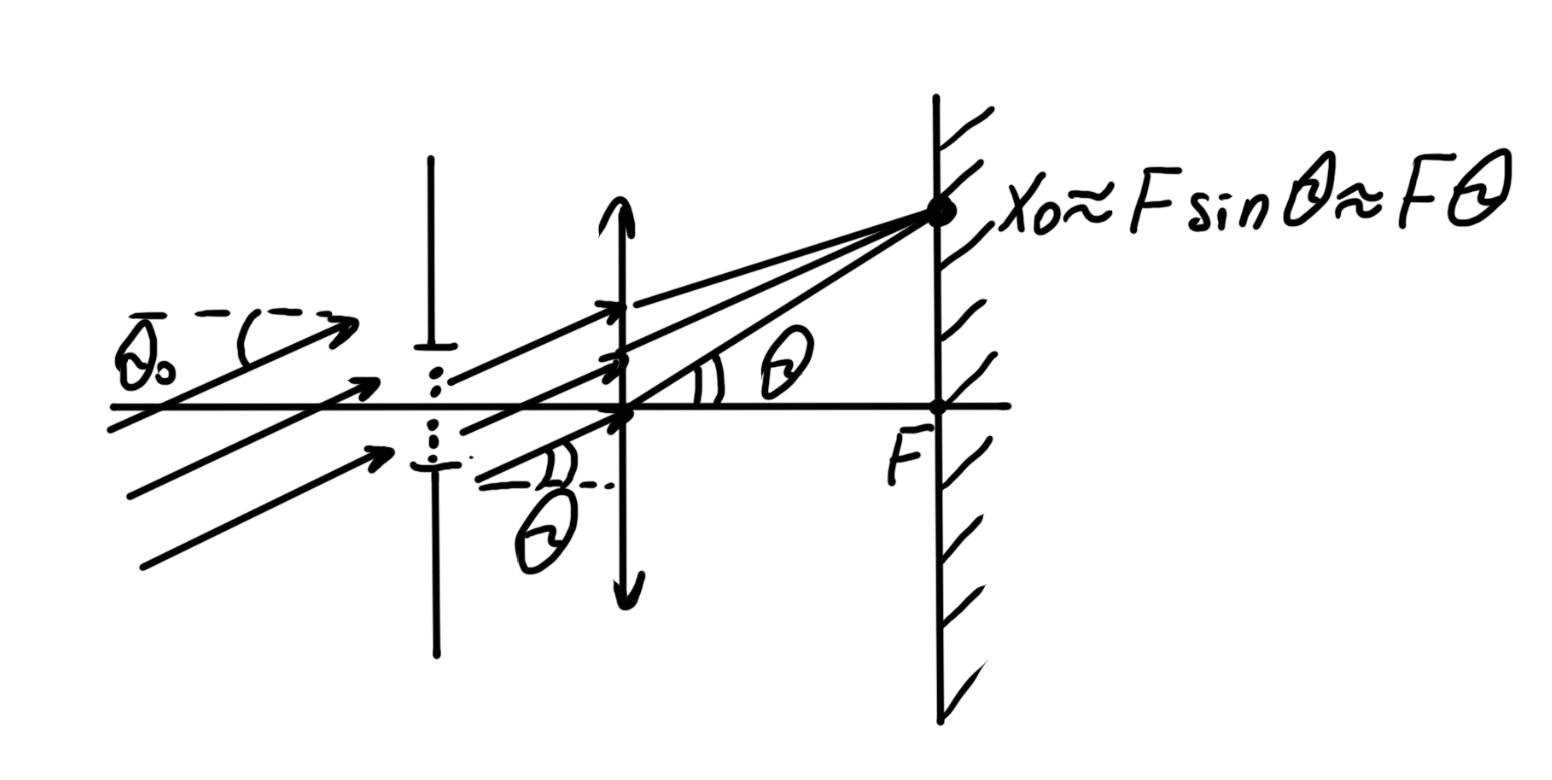
\includegraphics[width=0.6\textwidth]{/Users/vladbelousov/Desktop/Semestr_4-FP-NSU/ЭиО/Лекции_по_дням/image/137.png}
\end{center}

В случае наблюдения диффракционной картины в фокальной плоскости линзы \( \displaystyle  \frac{1}{R_p } \to  \frac{1}{F }   \), а \( \theta  \) остается тот же самый: \(\displaystyle  I = I_0 \frac{d ^2 }{\lambda F }\left( \frac{kd}{2 } (\sin \theta_0 - \sin \theta) \right) \cos  ^2 \theta   \) 

\section{Дифракционные решетки}

\textit{1. Щелевая решетка: } 

\begin{center}
    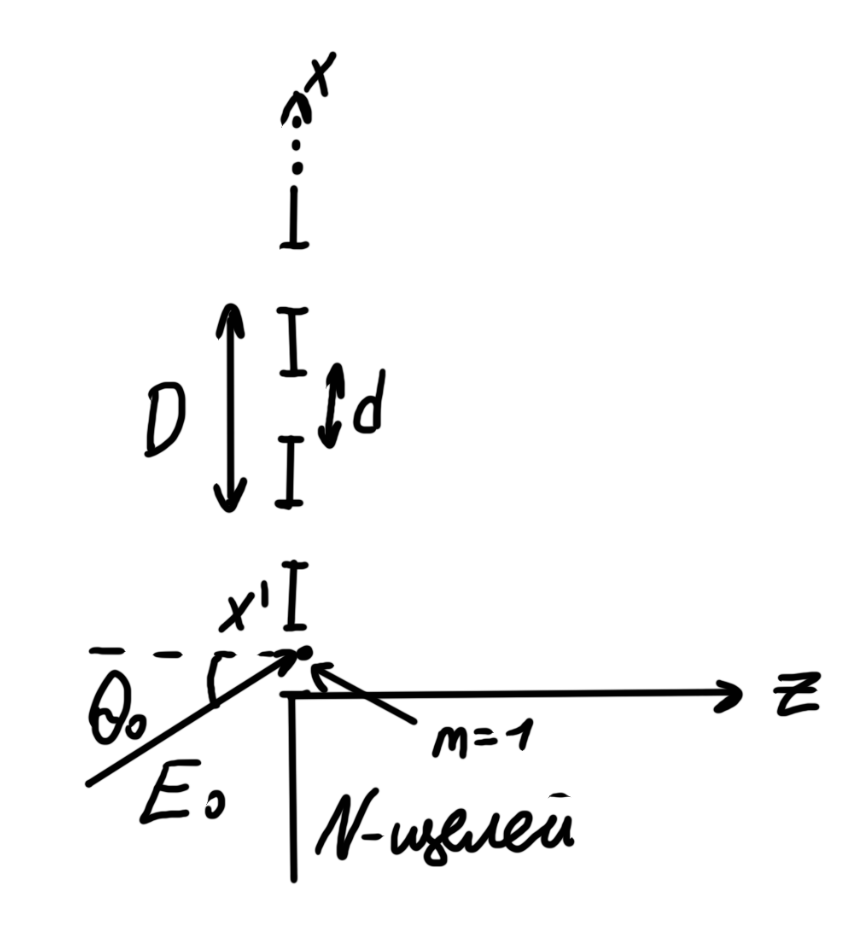
\includegraphics[width=0.4\textwidth]{/Users/vladbelousov/Desktop/Semestr_4-FP-NSU/ЭиО/Лекции_по_дням/image/138.png}
\end{center} 

\[ \hat{ E } (k_x ) = \frac{1}{\sqrt{2 \pi }} \int_{(m -1 )D}^{(m-1)D +d} E_0 e^{ i k (\sin  \theta_0 - \sin  \theta) x' } dx' = \frac{E_0}{\sqrt{2 \pi}} \sum_{m =1}^{N }  \frac{e^{i \Delta k_x ((m -1 )D + d)} - e^{i \Delta k_x (m -1 )D } }{i \Delta k_x } =     \] 
\[ =\frac{E_0}{\sqrt{2 \pi }} \frac{d e ^{i \Delta k_x d } -1 }{ 2 i \Delta k_x \frac{d}{2 }  } \sum_{m =1}^{N }  e^{ i \Delta k_x (m-1 )D } = \frac{d E_0}{\sqrt{2 \pi }}  e^{ i \Delta k_x \frac{d}{2} } \mathrm{sinc } \left( \Delta k_x \frac{d}{2}  \right)   \cdot\frac{e^{ i \Delta k_x N D} -1 }{e^{ i \Delta k_x N D  } -1 }   \] 
, где \( \Delta k_x  = k (\sin \theta_0 - \sin \theta) \) 

\[ I_p = \frac{\left\lvert  E_p \right\rvert ^2 }{2 } = \underbrace{\frac{d ^2 }{\lambda R_p } I_0 \mathrm{sinc } ^2 \left( \frac{kd}{2 } (\sin \theta_0 - \sin \theta) \right) \cos ^2 \theta}_{\text{дифракция на отдельной щели} } \cdot  \underbrace{\frac{\sin ^2 \displaystyle  \left(  \frac{kD}{2 } (\sin \theta_0 - \sin \theta) N \right)}{\sin  ^2 \displaystyle  \left( \frac{kD}{2 } (\sin \theta_0 - \sin \theta)  \right)}  }_{\text{интерференция полей от N-щелей} }   \] 
, где в конце дробь равна \( \frac{ \displaystyle  \sin  ^2 \frac{N \Delta \varphi }{2} }{\displaystyle \sin  ^2 \frac{ \Delta \varphi }{2} }  \). 

\begin{center}
    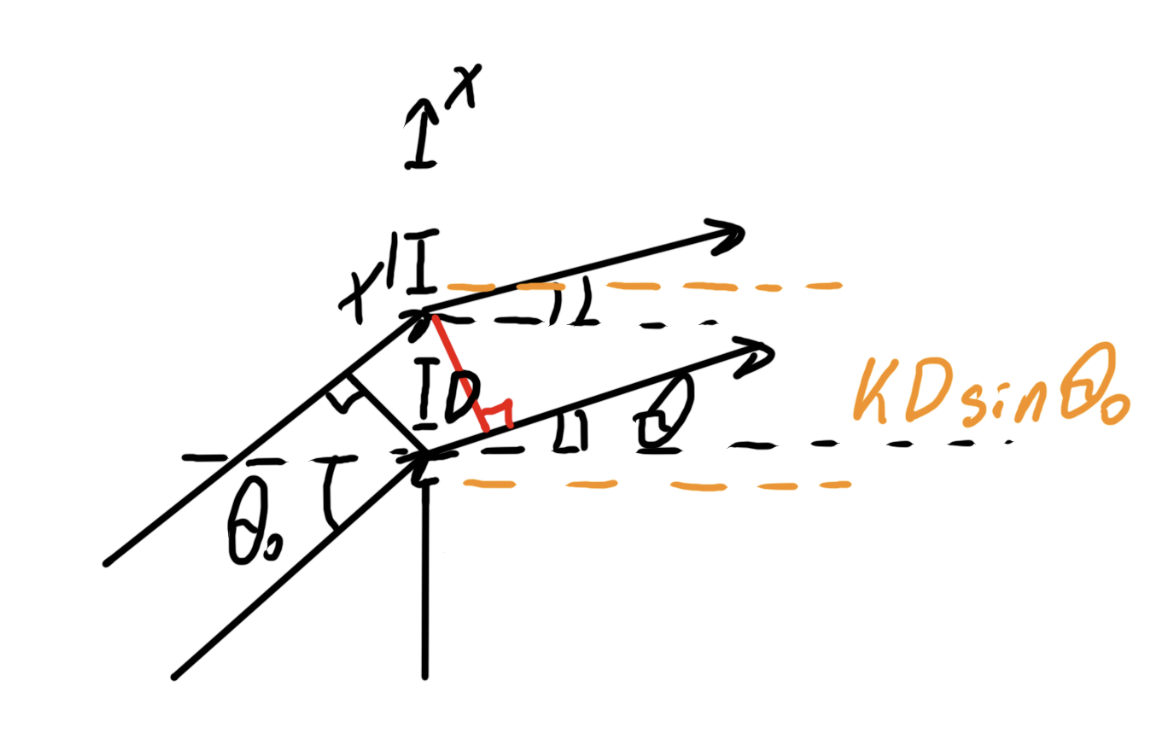
\includegraphics[width=0.5\textwidth]{/Users/vladbelousov/Desktop/Semestr_4-FP-NSU/ЭиО/Лекции_по_дням/image/139.png}
\end{center}
\[ \Delta \varphi = kD \sin \theta_0 - k D \sin  \theta \] 

\( \displaystyle   \frac{ \displaystyle  \sin  ^2 \frac{N \Delta \varphi }{2} }{\displaystyle \sin  ^2 \frac{ \Delta \varphi }{2} } \) - имеет главные максимумы в точках, где знаменатель = 0, то есть: \( \Delta \varphi = 2 \pi m , \text{ }  m = - \infty, \ldots, -1,0,1, \ldots, \infty  \) 
\[ kD (\sin \theta_0 - \sin  \theta_m ) = 2\pi m  \] 

Пусть \( \theta_m = \theta_0 + \Delta \theta_m : \) 

\[ \sin \theta_0 - \sin \theta_0 \cos  \Delta \theta_m - \cos \theta_0 \sin \Delta \theta_m = m \frac{\lambda}{D}  \] 
, где \( \displaystyle  \Delta \theta_m = m \frac{\lambda}{ D \cos \theta_0}  \). 

\begin{center}
    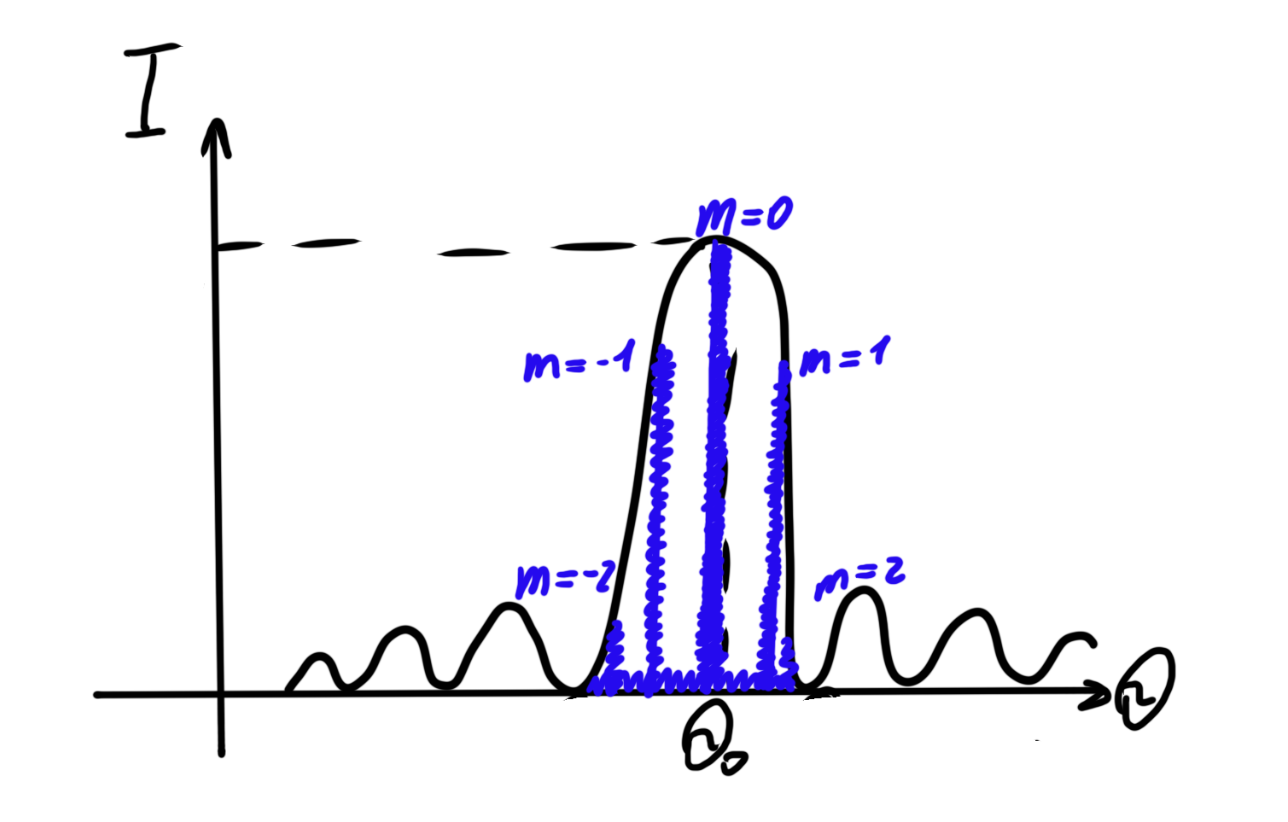
\includegraphics[width=0.5\textwidth]{/Users/vladbelousov/Desktop/Semestr_4-FP-NSU/ЭиО/Лекции_по_дням/image/140.png}
\end{center}

Ширина максимумов: 

\begin{center}
    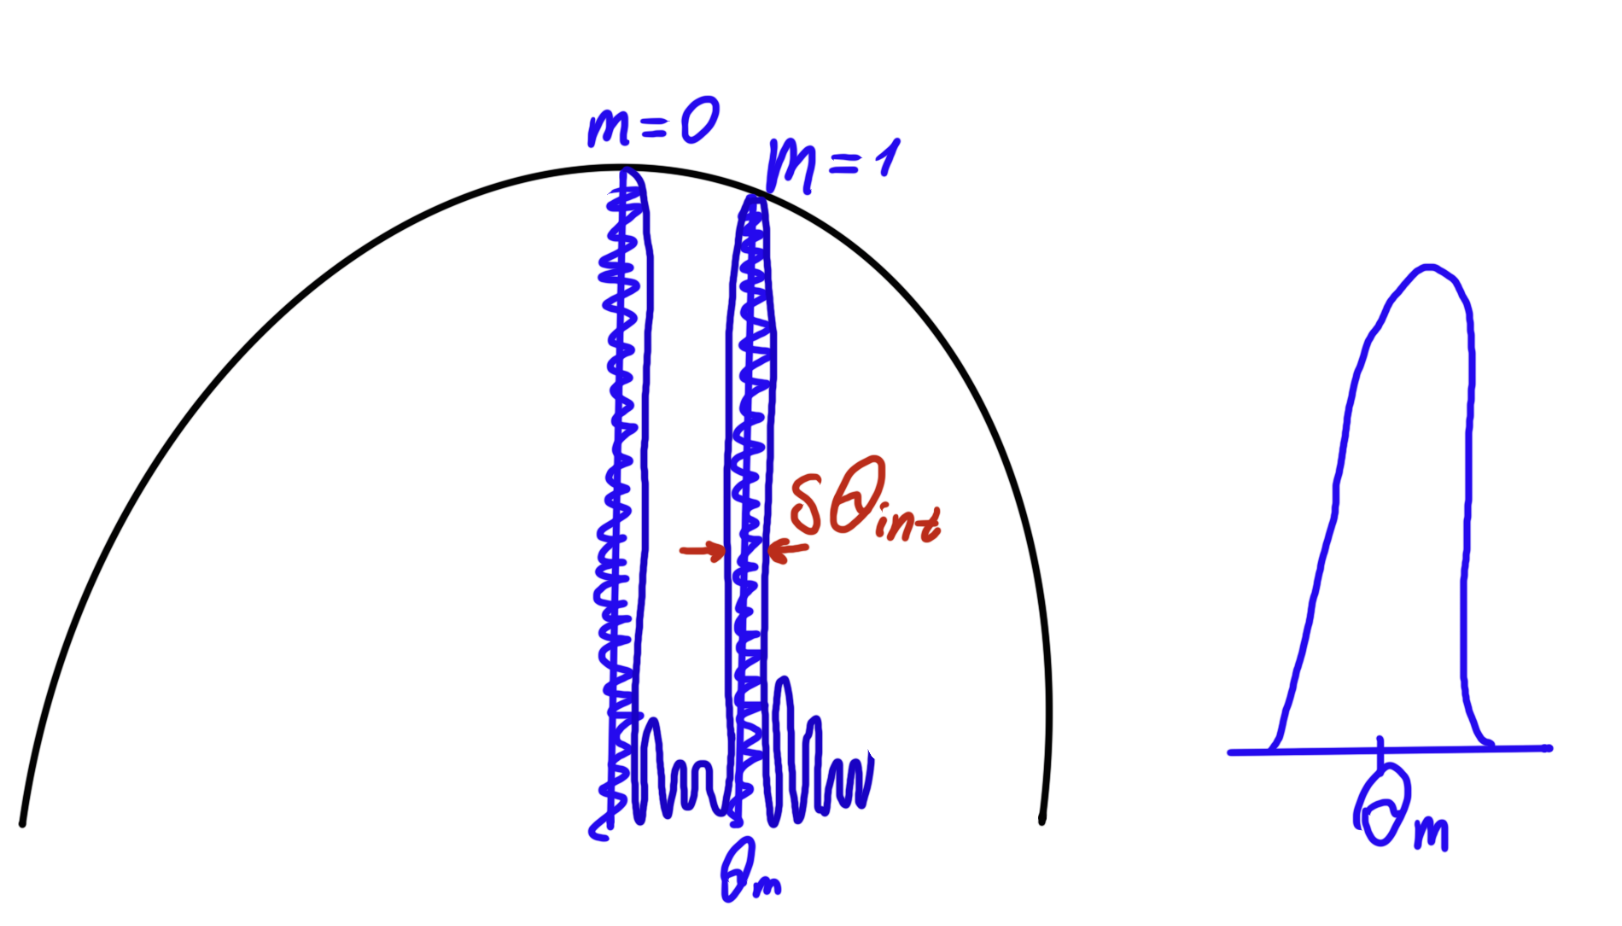
\includegraphics[width=0.4\textwidth]{/Users/vladbelousov/Desktop/Semestr_4-FP-NSU/ЭиО/Лекции_по_дням/image/141.png}
\end{center}

\( \delta \theta_{int } =   \)  угловое расстояние между главным максимум  и первым  интенсивности в 0. 

\[ \frac{N \Delta \varphi }{2 } \frac{N k D (\sin  \theta_0 - \sin (\theta_m + \sigma \theta_{ int } ))}{2 } = \frac{ - 2 \pi m N }{2 } \pm  \pi    \] 
\[ \frac{ N k D }{2 } ( \sin  \theta_0 - \sin  \theta_m \cos  \delta \theta_{ int }  - \cos  \theta_m  \sin \delta \theta_{ int }  ) = - m \pi N \pm  \pi  \] 
\[  \frac{k D }{2 } (\sin  \theta_0 - \sin \theta_m) = - m \pi \Rightarrow \frac{N k D }{2 }  \cos \theta_m \delta \theta_{ int }  = \pm  \pi\] 
\[ \delta \theta_{ int }  = \frac{\lambda}{D \cos  \theta_m }\frac{1}{N  }  \sim \frac{\lambda}{D \cos \theta_0 } \pm  \pi   \] 
, где \( \displaystyle  \frac{\lambda}{D \cos \theta_0} = \Delta \theta_{m + 1 }  - \Delta \theta_m  \) \\

\textit{2. Фазовые решетки: } 

\begin{center}
    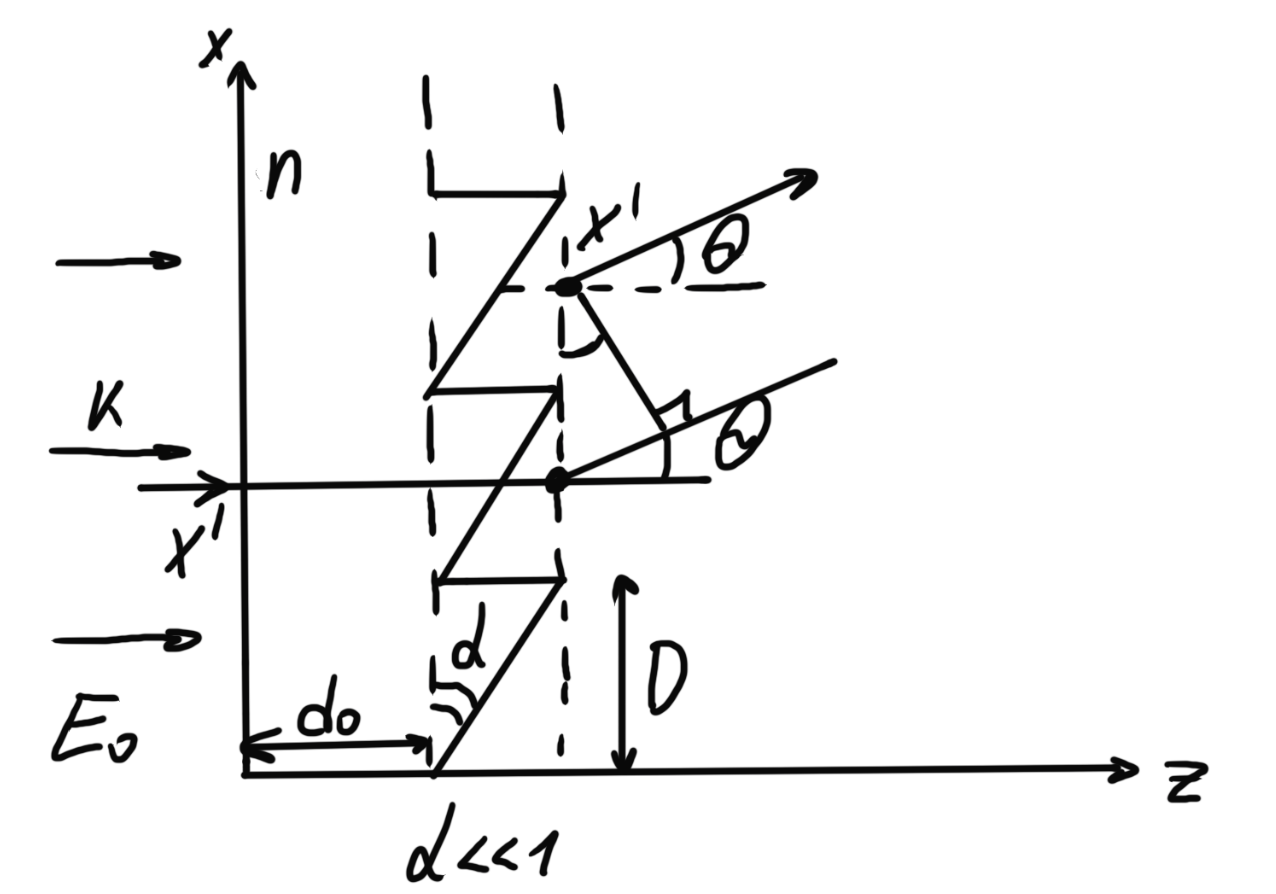
\includegraphics[width=0.4\textwidth]{/Users/vladbelousov/Desktop/Semestr_4-FP-NSU/ЭиО/Лекции_по_дням/image/142.png}
\end{center}

\[  \Delta \varphi = k \int n d S  = k [d_0 n + x' \alpha n + (D - x' )\alpha ] = \varphi_0 + k \alpha ( n-1 ) x' \] 

\[\kern-1cm \text{Одной ступеньки: } \hat{E } (k_x ) = \frac{1}{ \sqrt{ 2 \pi } } \int_{ 0 }^{D }  E_0 e^{ i \varphi_0 } e^{ i kja (n -1 ) x'  } e^{ - i k_x x' } dx ' = \frac{1}{\sqrt{2 \pi } } E_0 e^{i \varphi_0 } \int_{0 }^{D} e^{ i k (\alpha(n-1 )- \sin  \theta) x ' } dx ' =           \] 
\[ =\frac{E_0 D }{\sqrt{ 2\pi } }e^{i \varphi_0 } \frac{e^{ i \Delta k_x D } -1       }{2 i \Delta k_x \frac{D}{2} } = \frac{D}{\sqrt{2\pi } } E_0 e^{ i \varphi_0} e^{ i \Delta k_x \frac{D}{2} } \mathrm{sinc } \left(  \frac{kD}{2 } (\alpha(n-1 )- \sin \theta) \right)         \] 
, где \( \Delta k_x = k (\alpha (n-1 )- \sin \theta) \) 

\[ I_{\text{одной щели} } = I_0 \frac{D ^2 }{\lambda R_p } \mathrm{sinc } ^2 \left(  \frac{kD}{2}  (\alpha (n-1 ) \sin \theta ) \right) \cos  ^2 \theta   \] 
, где \( \alpha(n-1 ) \le \sin \theta_0 \) 

\[ \Delta \varphi_{\text{соседних зубов} } = k D \sin \theta  \] 

\[ I = I_0 \frac{ D ^2 }{\lambda R_p } \mathrm{sinc } ^2 \left( \frac{kD}{2} (\alpha(n-1 )- \sin \theta) \right) \cos ^2 \theta \cdot \frac{ \displaystyle  \sin ^2 \left( \frac{N k D \sin  \theta}{2}  \right)}{\displaystyle \sin  ^2 \left( \frac{ k D \sin  \theta}{2}  \right)}    \] 
, где \( R_p \to  F \) 

\begin{center}
    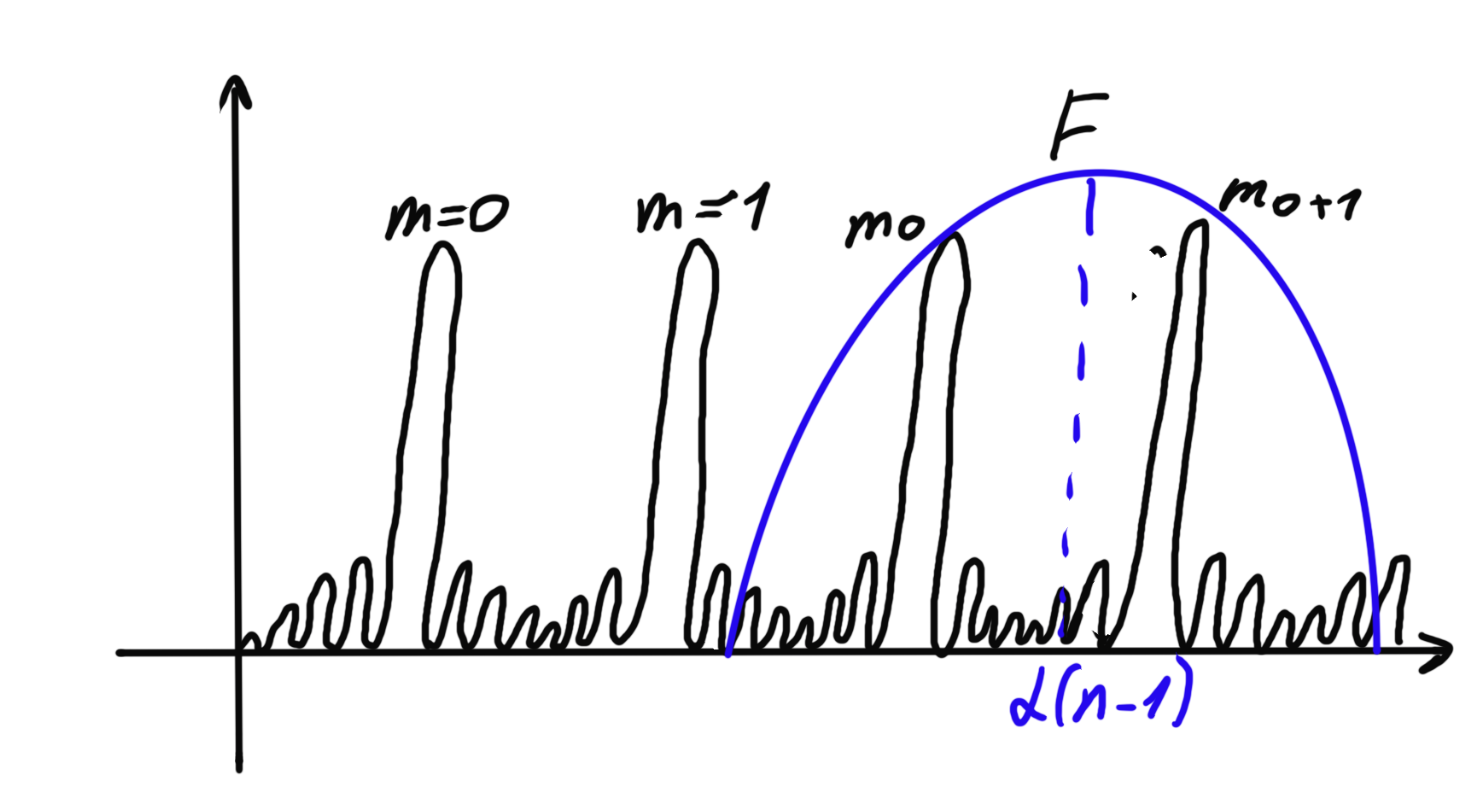
\includegraphics[width=0.5\textwidth]{/Users/vladbelousov/Desktop/Semestr_4-FP-NSU/ЭиО/Лекции_по_дням/image/143.png}
\end{center}
\(\displaystyle  R_{\lambda } = m_0 N = \frac{\lambda}{\delta \lambda}   \) 

%%-------------------------------%%

% Закрытие документа, если файл компилируется отдельно
\ifdefined\mainfile
    % Если это основной файл, не нужно заканчивать документ
\else
    \end{document}
\fi